% !TeX spellcheck = en_US
\section{Periodic table}
\begin{table}[ht!]
    \centering
    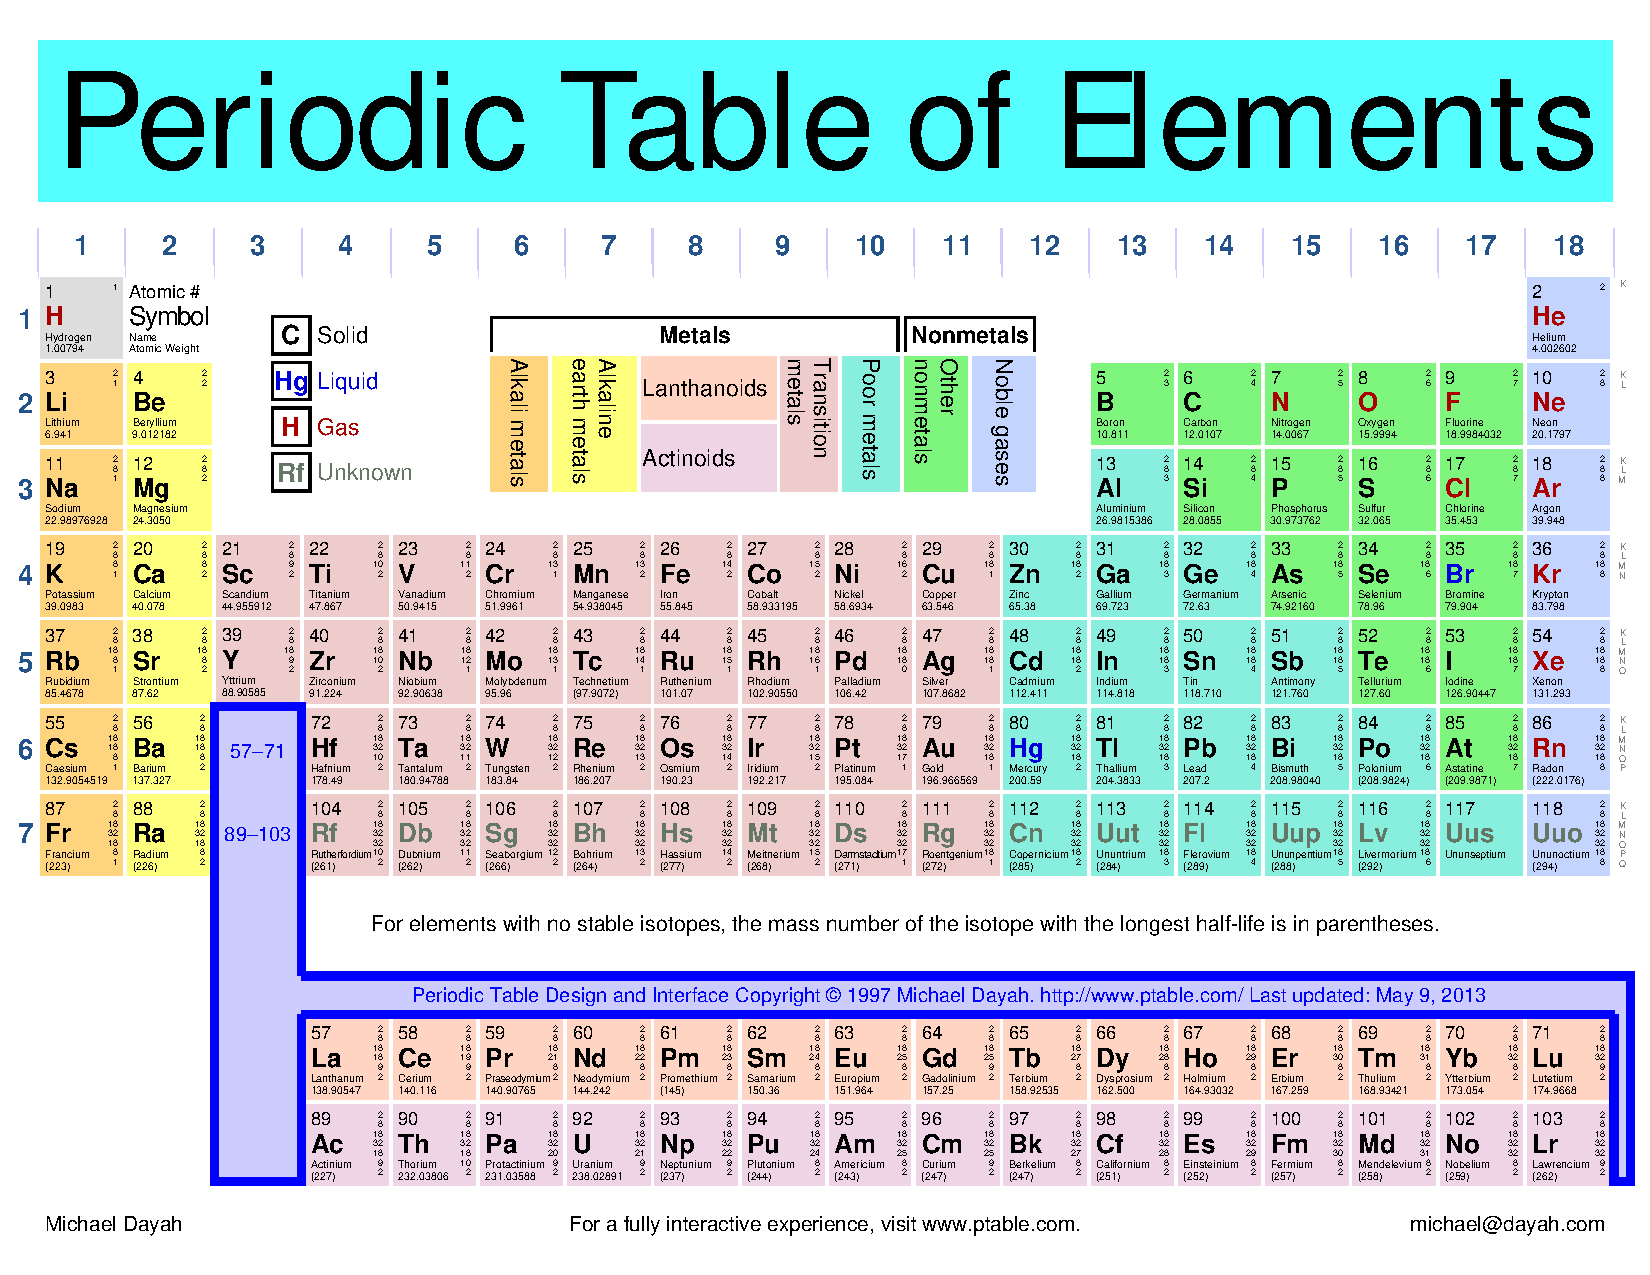
\includegraphics[height=0.9\linewidth,angle=90]{images/Periodic_Table.pdf}
    \caption{The periodic table of elements}
    \label{tab:app_periodictable}
\end{table}

\section{Resistivity and thermal coefficients for various metals}
\begin{table}[ht!]
    \centering
    \begin{tabular}{llll}
    \toprule
        Metal & $\rho_0$ (\si{\nano\ohm\meter}) & $\alpha_0$ (\si{1\per\kelvin}) & n \\ \midrule
        Aluminum, Al & 25.0 & 1/233 & \\
        Antimony, Sb & 38 & 1/196 & \\
        Copper, Cu & 15.7 & 1/232 & 1.15 \\
        Gold, Au & 22.8 & 1/251 & \\
        Indium, In & 78.0 & 1/196 & \\
        Platinum, Pt & 98 & 1/255 & 0.94 \\
        Silver, Ag & 14.6 & 1/244 & 1.11 \\
        Tantalum, Ta & 117 & 1/294 & 0.93 \\
        Tin, Sn & 110 & 1/217 & 1.11 \\
        Tungsten, W & 50 & 1/202 & 1.20 \\
        Iron, Fe & 84.0 & 1/152 & 1.80 \\
        Nickel, Ni & 59.0 & 1/125 & 1.72 \\
    \bottomrule
    \end{tabular} \\
    For non-magnetic metals, $n$ is close to unity.
    \caption{Resistivityand  thermal coefficient of resistivity for various metals}
    \label{app:resistivity}
\end{table}

\section{Hall coefficients}
\begin{table}[ht!]
    \centering
    \begin{tabular}{llll}
    \toprule
        Metal & $n$ (\si{\meter\tothe{-3}}) & $R_H$ (\si{\meter\tothe{3}\per\ampere\second}) & $\mu_h=|\sigma R_H|$ (\si{\square\meter\per\volt\second}) \\ \midrule
            & $\times 10^{28}$ & $\times 10^{-11}$ & $\times 10^{-4}$ \\
        Ag & 5.85 & -9.0 & 57 \\
        Al & 18.06 & -3.5 & 13 \\
        Au & 5.90 & -7.2 & 31 \\
        Be & 24.2 & +3.4 & ? \\
        Cu & 8.45 & -5.5 & 32 \\
        Ga & 15.3 & -6.3 & 3.6 \\
        In & 11.49 & -2.4 & 2.9 \\
        Mg & 8.60 & -9.4 & 22 \\
        Na & 2.56 & -25 & 53 \\
    \bottomrule
    \end{tabular}
    \caption{Hall coefficients of various metals}
    \label{app:Hall}
\end{table}

\section{Thermal conductivity}
\begin{table}[ht!]
    \centering
    \begin{tabular}{llllllll}
    \toprule
        \multicolumn{2}{c}{Pure metals} & \multicolumn{2}{c}{Metal alloys} & \multicolumn{2}{c}{Ceramics} & \multicolumn{2}{c}{Polymersmics} \\\midrule
        Nb & 52 & Stainless steel & 12-16 & Glass-borosilicate & 0.75 & PVC & 0.17 \\
        Fe & 80 & Bronce (95\% Cu - 5\% Sn) & 80 & Alumina (Al$_2$O$_3$) & 30 & Teflon & 0.25 \\
        Al & 250 & Brass (63\% Cu - 37\% Zn) & 125 & Beryllium oxyde & 260 & Polyethylene & 0.4 \\
        Cu & 390 && & Diamond & 1000 && \\
        Ag & 420 && && && \\
    \bottomrule
    \end{tabular}
    \caption{Thermal conductivity $\kappa$ (\si{\watt\per\meter\kelvin}) for various materials}
    \label{app:thermalcond}
\end{table}

\section{Fermi energy and work function}
\begin{table}[ht!]
    \centering
    \begin{tabular}{lllllllll}
    \toprule
        & \multicolumn{8}{c}{Metal}\\ \cmidrule{2-9}
        & Ag & Al & Au & Cs & Cu & Li & Mg & Na \\ \midrule
        $\varPhi$ (\si{\electronvolt}) & 4.5 & 4.28 & 5.0 & 2.14 & 4.65 & 2.3 & 3.7 & 2.75 \\
        $E_{F0}$ (\si{\electronvolt}) & 5.5 & 11.7 & 5.5 & 1.58 & 7.0 & 4.7 & 7.1 & 3.2 \\
    \bottomrule
    \end{tabular}
    \caption{Fermi energy and work function of selected metals}
    \label{app:fermienergy}
\end{table}

\section{Effective mass}
\begin{table}[htbp]
    \centering
    \begin{tabular}{lcccccccccc}
    \toprule
    Metal & Ag & Au & Bi & Cu & K & Li & Na & Ni & Pt & Zn \\
    $\frac{m_e^*}{m_e}$ & 0.99 & 1.10 & 0.047 & 1.01 & 1.12 & 1.28 & 1.2 & 28 & 13 & 0.85 \\
    \bottomrule
    \end{tabular}
    \caption{Effective mass $m_e^*$ of electrons in some metals}
    \label{app:effectivemass}
\end{table}

%TODO: achtung newpage!!
\newpage

\section{Seebeck coefficients}
\begin{table}[ht!]
    \centering
    \begin{tabular}{lllll}
    Metal & S at \SI{0}{\degreeCelsius} (\si{\micro\volt\per\kelvin}) & S at \SI{27}{\degreeCelsius} (\si{\micro\volt\per\kelvin}) & $E_F$ (\si{\eV}) & x \\ \toprule
    Al   & -1.6    & -1.8   & 11.6 & 2.78    \\
    Au  & +1.79 & +1.94 & 5.5   & -1.48  \\
    Cu  & +1.70 & +1.84 & 7.0   & -1.79  \\
    K    &            &  -12.5 & 2.0   & 3.8      \\
    Li   & +14     &           & 4.7    & -9.7    \\
    Mg & -1.3    &           & 7.1    & 1.38     \\
    Na  &            & -5      & 3.1   & 2.2        \\
    Pd  & -9.00   & -9.99 &         &             \\
    Pt  & -4.45    & -5.28 &         &             \\ \bottomrule
    \end{tabular}
    \caption{Seebeck coefficients of selected materials. (Source: Kasap, Table 4.3)}
    \label{app:seebeck}
\end{table}

\section{Semiconductor properties}
\begin{table}[ht!]
    \centering
    \begin{tabularx}{\linewidth}{lcccccccXXc}
    \toprule
        & $E_g$ & $\chi$ & $N_c$ & $N_v$ & $n_i$ & $\mu_e$ & $\mu_h$ & & & \\
        & (\si{\electronvolt}) & (\si{\electronvolt}) & (\si{\centi\meter\tothe{-3}}) & (\si{\centi\meter\tothe{-3}}) & (\si{\centi\meter\tothe{-3}}) & (\si{\square\centi\meter\per\volt\second}) & (\si{\square\centi\meter\per\volt\second}) & $m_e^*/m_e$ & $m_h^*/m_e$ & $\varepsilon_r$ \\ \midrule
        Ge & 0.66 & 4.13 & \num{1.04e19} & \num{6.0e18} & \num{2.3e13} & 3900 & 1900 & 0.12a 0.56b & 0.23a 0.40b & 16 \\
        Si & 1.10 & 4.01 & \num{2.8e19} & \num{1.2e19} & \num{1.0e10} & 1350 & 450 & 0.26a 1.08b & 0.38a 0.60b & 11.9 \\
        GaAs & 1.42 & 4.07 & \num{4.7e17} & \num{7e18} & \num{2.1e6} & 8500 & 400 & 0.067a,b & 0.40a 0.50b & 13.1 \\
    \bottomrule
    \end{tabularx}
    \caption{Selected typical properties of Ge, Si and GaAs at \SI{300}{\kelvin}}
    \label{app:semiconductors}
\end{table}

%TODO: achtung newpage
\newpage

\section{Electronic polarizability}
\begin{table}[ht!]
    \centering
    \begin{tabular}{lllllll}
    \toprule
        & \multicolumn{6}{c}{Atom} \\ \cmidrule{2-7}
        & He & Ne & Ar & Kr & Xe & Rn \\ \midrule
        Z & 2 & 10 & 29 & 36 & 56 & \\
        $\alpha_e$ (\SI{e-40}{\farad\per\square\meter}) & 0.18 & 0.45 & 1.7 & 2.7 & 4.4 & 5.9 \\
        $f_0$ \SI{e15}{\hertz}) & 8.90 & 12.6 & 8.69 & 9.76 & 9.36 & 10.2 \\
    \bottomrule
    \end{tabular}
    \caption{Electronic polarizability $\alpha_e$ dependence on $Z$ for the inert element atoms}
    \label{app:polarizability}
\end{table}

\section{Piezoelectric coefficient}
\begin{table}[ht!]
    \centering
    \begin{tabularx}{\linewidth}{p{5cm}llX}
    \toprule
        Crystal & d (\si{\meter\per\volt}) & k & Comment \\ \midrule
        Quartz (crystal $SiO_2$) & \num{2.3e-12} & 0.1 & Crystal oscillators, ultrasonic transducers, delay lines, filters. \\
        Rochelle salt \newline ($NaKC_4H_4O_63H_2O$) & \num{350e-12} & 0.78 & \\
        Barium titanate ($BaTiO_3$) & \num{190e-12} & 0.49 & Accelerometers \\
        PZT, Lead zirconate titanate ($PbTi_{1-x}Zr_xO_3$) & \num{480e-12} & 0.72 & Wide range of applications including earphones, microphones, spark generators, displacement transducers, accelerometers. \\
        Polyvinylidenefluoride (PVDF) & \num{18.2e-12} & & Must be poled, heated, put in an electric field and then cooled. Large area and inexpensive. \\
    \bottomrule
    \end{tabularx}
    \caption{Piezoelectric coefficient and electromechanical coupling factor of some piezo materials}
    \label{app:piezo}
\end{table}

%TODO: achtung newpage
\newpage

\section{Pyroelectric and ferroelectric properties}
\begin{table}[ht!]
    \centering
    \begin{tabular}{p{3cm}p{3cm}c>{\centering\arraybackslash}m{3cm}>{\centering\arraybackslash}m{3cm}}
    \toprule
        Material & $\varepsilon_r'$ & $\tan\delta$ & Pyroelectric coefficient $p$ (\SI{e-6}{\coulomb\per\square\meter\kelvin}) & Curie\newline temperature (\si{\celsius})\\ \midrule
        $BaTiO_3$ & $4100\:\bot$ polar axis \newline $160\:||$ polar axis  & \num{7e-3} & 20 & 130 \\
        $LiTaO_3$ & 47 & \num{5e-3} & 230 & 610 \\
        PZT modified for pyroelectric & 290 & \num{2.7e-3} & 380 & 230 \\
        PVDF, polymer & 12 & 0.01 & 27 & 80 \\
    \bottomrule
    \end{tabular}
    \caption{Some pyroelectric and ferroelectric crystals and typical properties}
    \label{app:pyroelectric}
\end{table}